\section{Тестирование и оценка эффективности}

\subsection{Тестирование функциональности}
Для проверки корректной работы голосового помощника был проведен ряд тестов. Основное внимание уделялось проверке реакции системы на ключевое слово и последующее выполнение команд. 

Срабатывани голосового помошника и выполнения команды только после ключевого слова Алиса можно увидеть на рисунке \ref{fig:test1}

\begin{figure}[H]
	\centering
	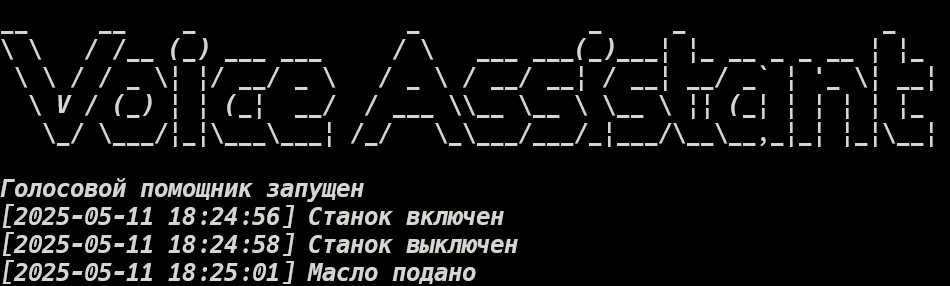
\includegraphics[scale=0.8]{test1.jpg}
	\caption{Тестированя срабатывания голосового помощника по ключевому слову Алиса}
	\label{fig:test1}
\end{figure}
Данный рисунок говорит о том голосовой помощник производит распознование команд коректно и реагирует на ключевое слово Алиса и дальше ждет ввода конкретной команды для распознования и обработки.


Для оценки устойчивости работы голосового помощника в условиях фоновых шумов было проведено тестирование, имитирующее реальную эксплуатацию устройства. Целью испытания являлась проверка корректности распознавания голосовых команд при наличии посторонних звуков и искажённых обращений. В рамках эксперимента были созданы помехи, затрудняющие распознавание, такие как работающий телевизор и произнесение случайных фраз, в том числе содержащих ключевое слово «Алиса» с некорректными командами, а также фразы без ключевого слова.

\begin{figure}[H]
	\centering
	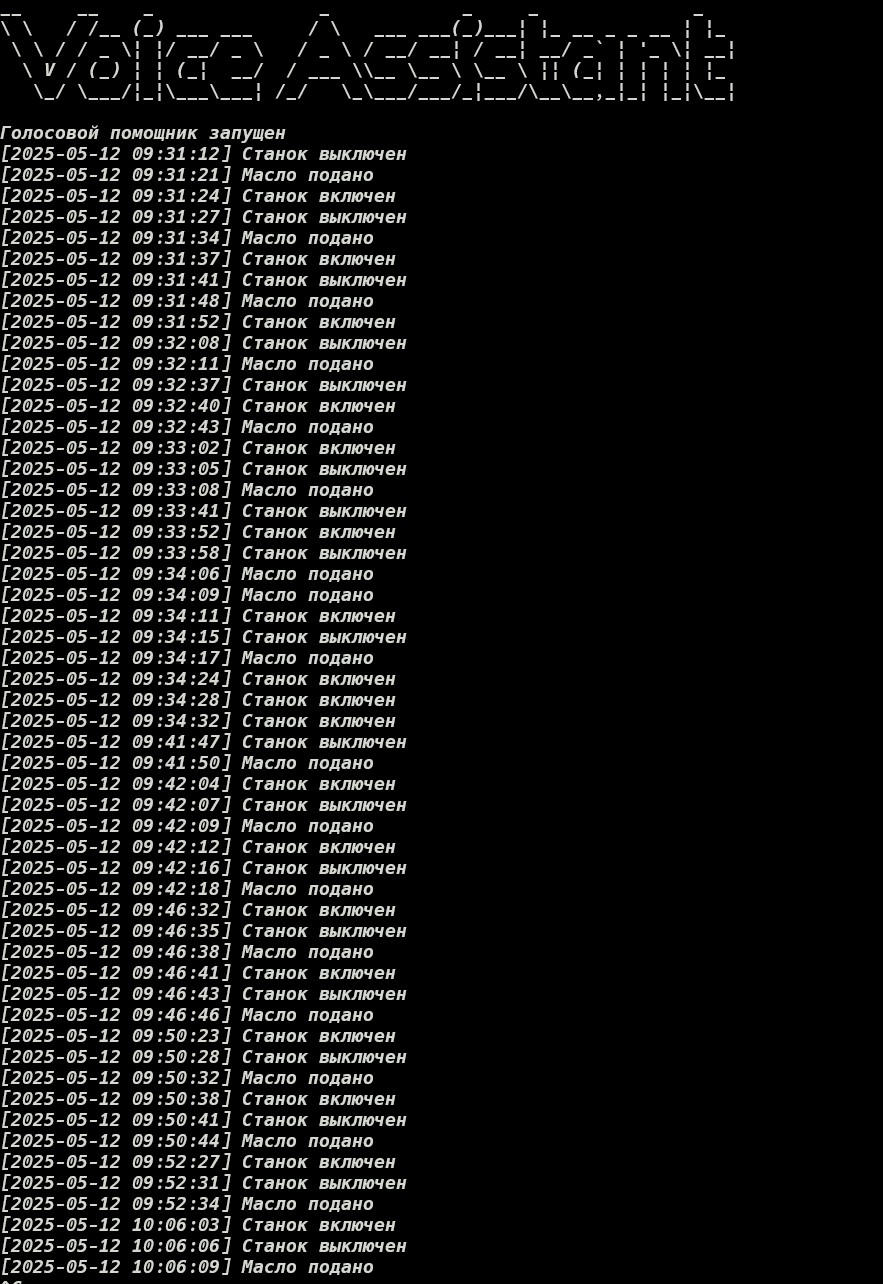
\includegraphics[scale=0.9]{test2_full.jpg}
	\caption{Вывод команд при работе голосового помощника}
	\label{fig:test2}
\end{figure}
В течение 35 минут голосовой помощник демонстрировал стабильную работу, корректно реагируя на валидные команды и игнорируя случайные фразы, не относящиеся к управлению. Выводы работы голосового помощника при тестировании приведены на рисунке \ref{fig:test2}.

\subsection{Оценка эффективности}

Для объективного анализа нагрузки голосового помошника на одноплатный компьютер был проведён эксперимент с использованием двух поколений аппаратных платформ:
\begin{itemize}
	\item Raspberry Pi 2 Model B Rev 1.1;
	\item Raspberry Pi 4 Model B Rev 1.5.
\end{itemize}

Конфигурацию Raspberry Pi 2 Model B Rev 1.1 можно увидеть используя программу fastfetch вывод программы представлен на рисунке \ref{fig:fastfetch_RaspberryPi2}

\begin{figure}[H]
	\centering
	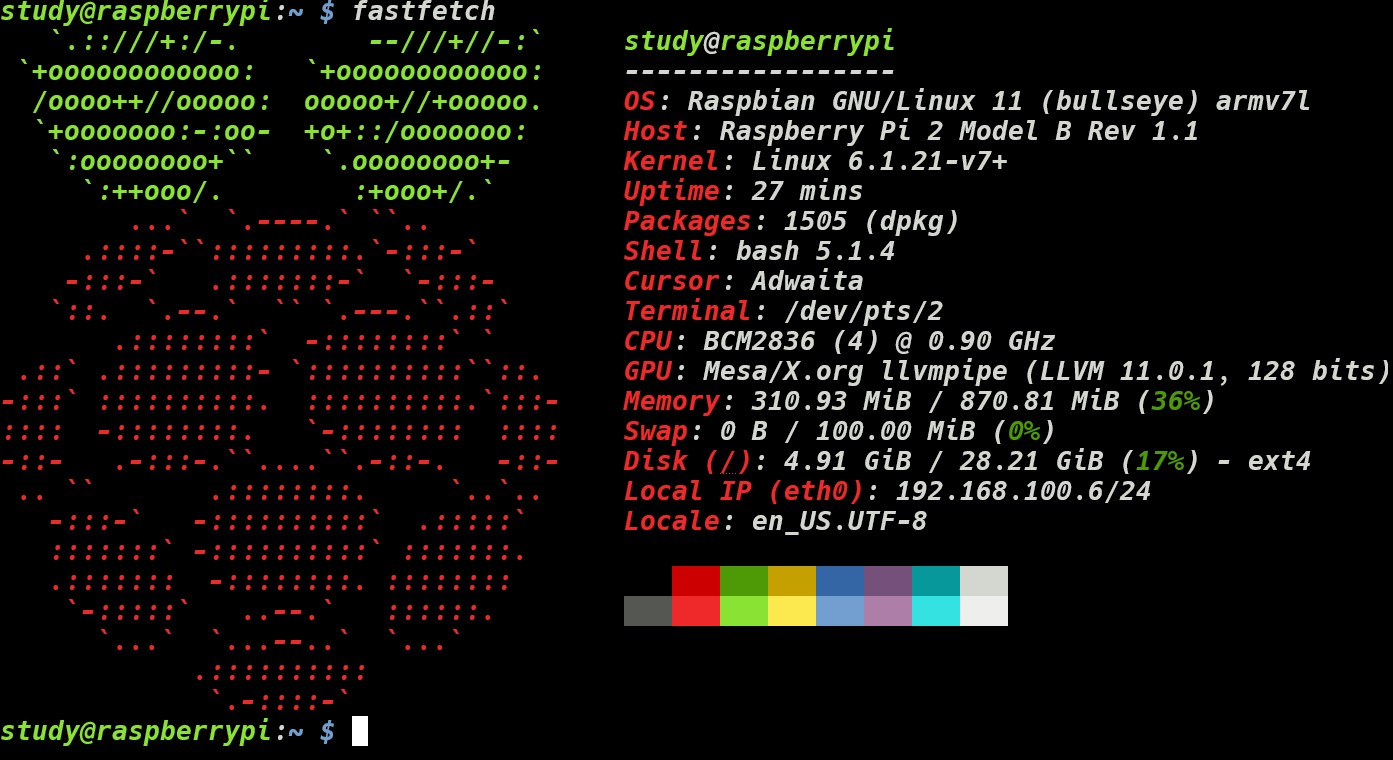
\includegraphics[scale=0.6]{fastfetch_RaspberryPi2.jpg}
	\caption{Вывод программы fastfetch}
	\label{fig:fastfetch_RaspberryPi2}
\end{figure}
Данная команда дает подробный вывод что именно установлено и что использует одноплатный компьютер

Для анализа потребления ресурсов голосовым помощником была запущена команда btop часть вывода этой команды показана на рисунке \ref{fig:useMemoryRaspberryPi2}

\begin{figure}[H]
	\centering
	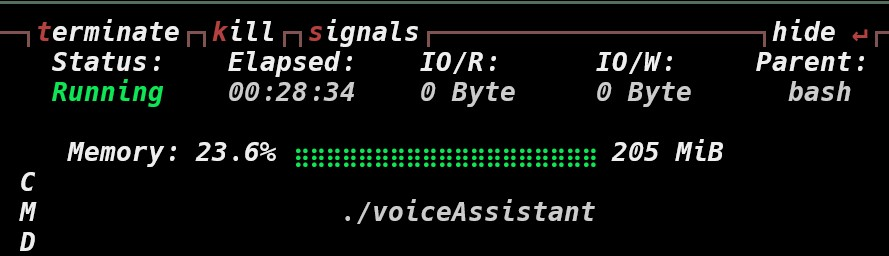
\includegraphics[scale=0.9]{useMemoryRaspberryPi2.jpg}
	\caption{Вывод программы btop о используемой памяти голосовым помощником}
	\label{fig:useMemoryRaspberryPi2}
\end{figure}
Данный рисунок демонстрирует время работы голосового помощника и используемую им память 

Конфигурацию Raspberry Pi 4 Model B Rev 1.5 можно увидеть используя программу fastfetch вывод программы представлен на рисунке \ref{fig:fastfetch_RaspberryPi4}

\begin{figure}[H]
	\centering
	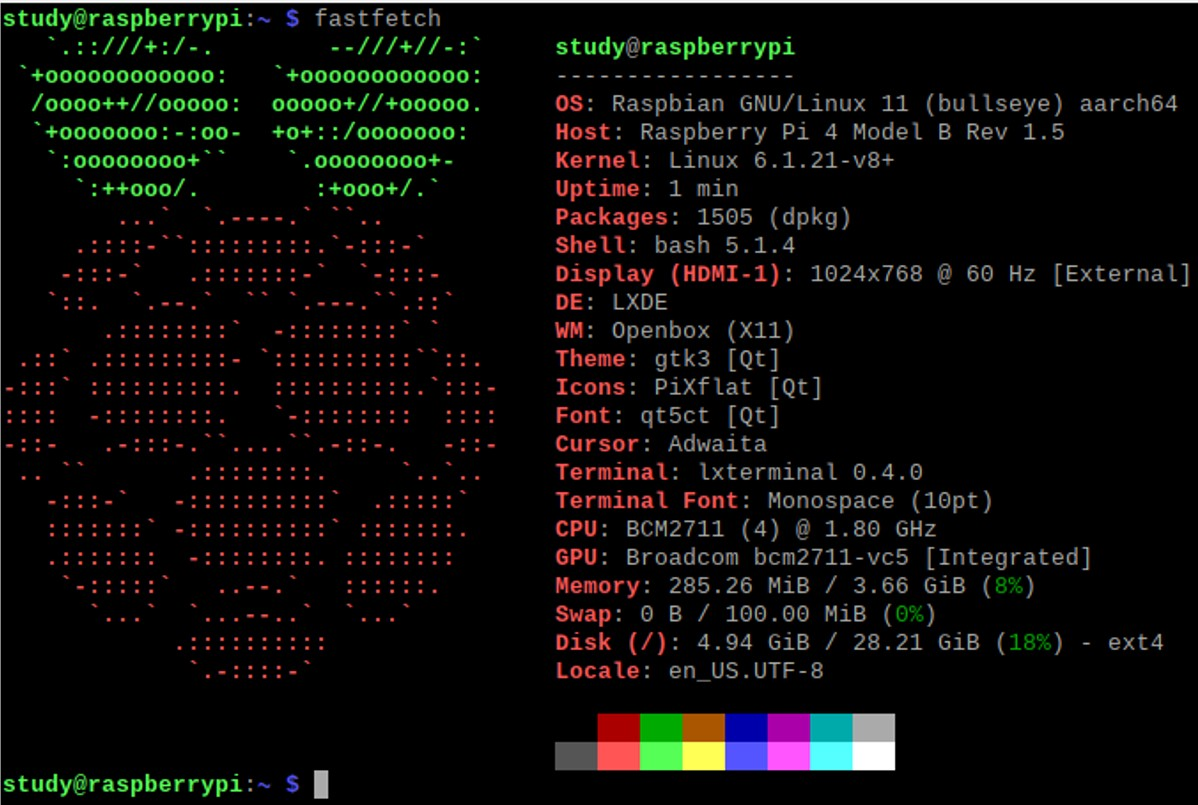
\includegraphics[scale=0.6]{fastfetch_RaspberryPi4.jpg}
	\caption{Вывод программы fastfetch}
	\label{fig:fastfetch_RaspberryPi4}
\end{figure}
Данная команда дает подробный вывод что именно установлено и что использует одноплатный компьютер

Для анализа потребления ресурсов голосовым помощником была запущена команда btop часть вывода этой команды показана на рисунке \ref{fig:useMemoryRaspberryPi4}

\begin{figure}[H]
	\centering
	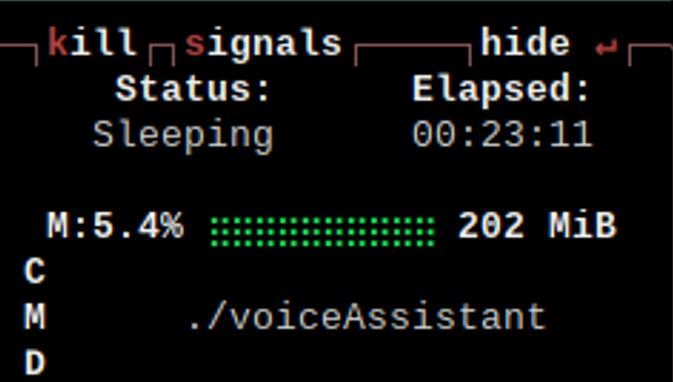
\includegraphics[scale=0.9]{useMemoryRaspberryPi4.jpg}
	\caption{Вывод программы btop о используемой памяти голосовыйм помошником}
	\label{fig:useMemoryRaspberryPi4}
\end{figure}
Данный рисунок демонстрирует время работы голосового помощника и используемую им память 

Все данные представленые на рисунках отображены в таблице 4.1

\begin{table}[H]
	\caption{Используемые ресурсы при работе голосового помощника}
	\centering 
	\begin{tblr}{
			width=\textwidth,
			colspec={X[4,l]|X[1.5,c,m]|X[1.5,c,m]},
			cell{3-11}{1} = {l},  % Объединенные ячейки (строки 3-11, столбец 1) - по левому краю
			vlines,
		}
		\hline 
		\SetCell[r=2]{c} Модель одноплатного компьютера & \SetCell[c=2]{c} Используемые ресурсы
		&   \\ 
		\hline  
		& CPU & RAM \\
		\hline  
		1 Raspberry Pi 2 Model B Rev 1.1  & 10-20\%  & 205Mb  \\ 
		\hline  
		2 Raspberry Pi 4 Model B Rev 1.5 & 2-5\% & 202Mb \\ 
		\hline  
	\end{tblr}
\end{table}

На основании данных таблицы видно, что голосовой помощник предъявляет сравнительно невысокие требования к вычислительным ресурсам одноплатного компьютера.

Таким образом, можно сделать вывод, что производительность устройства напрямую влияет на загрузку процессора: с увеличением вычислительных возможностей, как это наблюдается при переходе от Raspberry Pi 2 к Raspberry Pi 4, нагрузка на CPU существенно уменьшается. При этом объём потребляемой оперативной памяти практически не изменяется, оставаясь в пределах 200–205 МБ, что свидетельствует о стабильном объёме потребляемых приложением ресурсов. В целом голосовой помощник способен корректно функционировать даже на устаревших моделях одноплатных компьютеров, однако использование более производительных решений позволяет снизить нагрузку на процессор и повысить общую отзывчивость системы.

\newpage
